%------------------------------------------------------------------------
%Editar Diplomado
\hypertarget{cv:eliminarColaborador}{\section{Eliminar Colaborador}} \label{sec:eliminarColaborador}

	Esta funcionalidad le permitirá eliminar un colaborador innecesario o incorrecto. Para eliminar un colaborador es necesario que no se encuentre asignado a ningún proyecto ya sea como líder o analista.

		\subsection{Procedimiento}

			%Pasos de procedimiento
			\begin{enumerate}
	
			\item Oprima el botón \IUBotonEliminar{} de un registro existente de la pantalla \ref{fig:GestionarColaboradores} ''Gestionar Colaboradores''.
	
			\item Se mostrará el mensaje \ref{fig:confirmaEliminaColaborador} sobre la pantalla \ref{fig:GestionarColaboradores} ''Gestionar Colaboradores''.
			
			%Pantalla
			\begin{figure}[htbp!]
				\begin{center}
					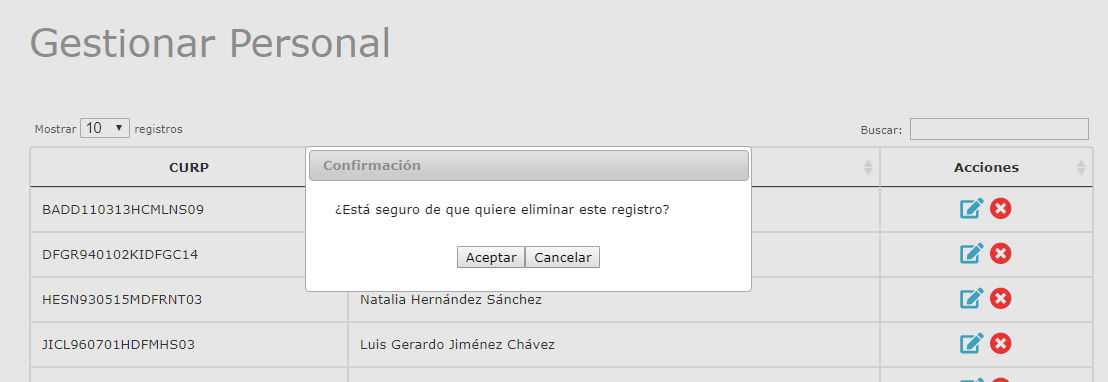
\includegraphics[scale=0.6]{roles/administrador/colaboradores/gestionarColaboradores/pantallas/IU3-3MSG10}
					\caption{MSG de Confirmación}
					\label{fig:confirmaEliminaColaborador}
				\end{center}
			\end{figure}
						
			\item Oprima el botón \IUAceptar.
			
			\item Se mostrará el mensaje \ref{fig:colaboradorEliminado} en la pantalla \ref{fig:GestionarColaboradores} ''Gestionar Colaboradores''.
			
			\begin{figure}[htbp!]
				\begin{center}
					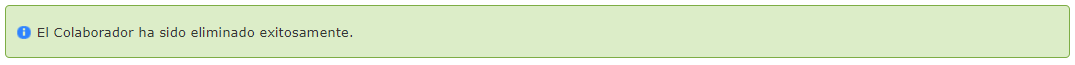
\includegraphics[scale=0.6]{roles/administrador/colaboradores/gestionarColaboradores/pantallas/IU3-3MSG1}
					\caption{MSG: Colaborador Eliminado}
					\label{fig:colaboradorEliminado}
				\end{center}
			\end{figure}
			\end{enumerate}